\documentclass{article}
\usepackage[english]{babel}
\usepackage[letterpaper,top=2cm,bottom=2cm,left=3cm,right=3cm,marginparwidth=1.75cm]{geometry}
\usepackage{amsmath}
\usepackage{graphicx}
\usepackage[colorlinks=true, allcolors=blue]{hyperref}
\usepackage{svg}
\usepackage{array}
\usepackage{float}
\usepackage{minted}
\usepackage{cleveref}
\usepackage{caption}
\usepackage{csquotes}
\usepackage[sorting=none]{biblatex}

\addbibresource{references.bib}

\setminted{
    autogobble,
    breaklines
}
% Create a new environment for breaking code listings across pages.
\newenvironment{longlisting}{\captionsetup{type=listing}}{}

\title{VGA On Zedboard}
\author{Jaeho Cho}

\begin{document}

\maketitle

\section{VGA Peripheral}

\subsection{Display}

\begin{figure}[hb]
    \centering
    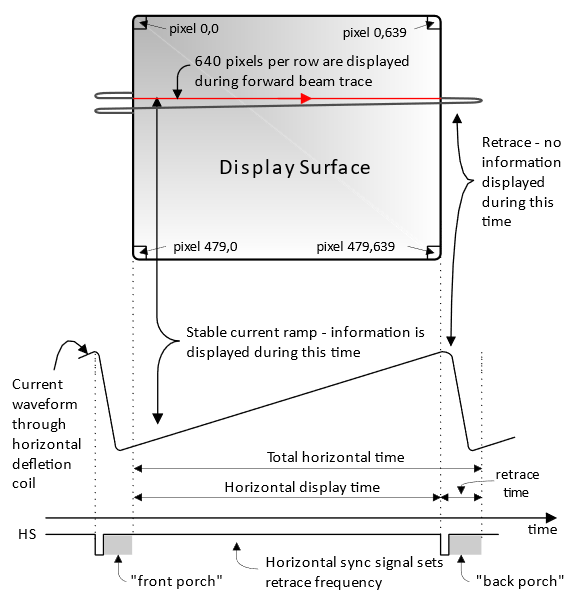
\includegraphics[width=0.75\linewidth]{CRT Operation and Timing.png}
    \caption{CRT Operation and Timing}
    \label{fig:CRT Op}
\end{figure}

The VGA display operates on a 640 x 480 pixel grid where pixel data is received serially as analog input, with timing signals controlling the rendering of the image. Figure \cref{fig:CRT Op} illustrates the timing in CRT displays, this involves a forward beam trace that lights up each pixel line-by-line, with synchronization provided by horizontal and vertical sync pulses. Key timing elements include the front porch, the interval between the end of active video and the start of the sync pulse, and the back porch, the time between the end of the sync pulse and the start of the next active video. Modern LCDs replace the beam trace with direct pixel addressing while maintaining the same VGA timing principles. The synchronization signals still play a critical role, ensuring pixel data is properly sequenced and mapped to the display grid without artifacts, even though the scanning process is no longer physical. This compatibility enables smooth rendering of video on both legacy and modern displays.

\subsection{Protocol}
\label{subsec:VGA Protocol}

The VGA controller protocol consists of three primary components: the clock generator, the timing generator, and the color output logic. The clock generator produces a pixel clock, synchronized to the display's refresh rate, using a clocking wizard or divider circuit. The timing generator includes horizontal and vertical counters that create the synchronization signals (HSYNC and VSYNC) based on the VGA standard. These counters manage the active video region (visible pixels) and blanking intervals, ensuring proper display refresh. The color output logic controls the RGB signals, outputting digital color values during the active video region to produce the desired image on the screen.

\subsection{Connector}

\begin{figure}[hb]
    \centering
    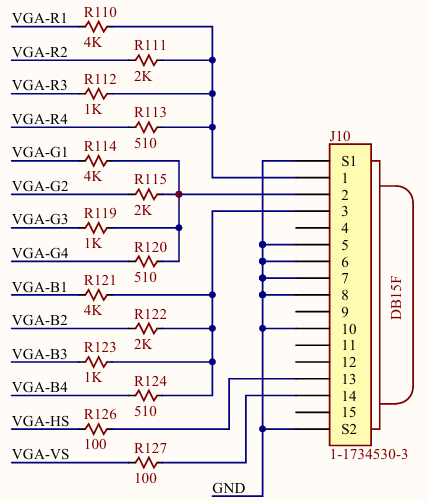
\includegraphics[width=0.5\linewidth]{VGA Interface Schematic.png}
    \caption{VGA Interface Schematic\cite{noauthor_zedboard_nodate} }
    \label{fig:VGA Sch}
\end{figure}

This schematic represents the Zedboard's VGA interface, connecting digital RGB (\verb|VGA-R|, \verb|VGA-G|, \verb|VGA-B|) and synchronization signals (\verb|VGA-HS|, \verb|VGA-VS|) to a \verb|DB15| VGA connector for output to a monitor. The RGB signals pass through a resistor ladder (\verb|R110|-\verb|R124|), converting digital signals into analog voltage levels (0–0.7\,V). The Hsync and Vsync signals are set low (active state) during the synchronization pulse period, indicating the start of a new line (for Hsync) or a new frame (for Vsync). They return to high (inactive state) during the rest of the line or frame to allow the display to continue scanning and drawing the image.

\begin{figure}[H]
    \centering
    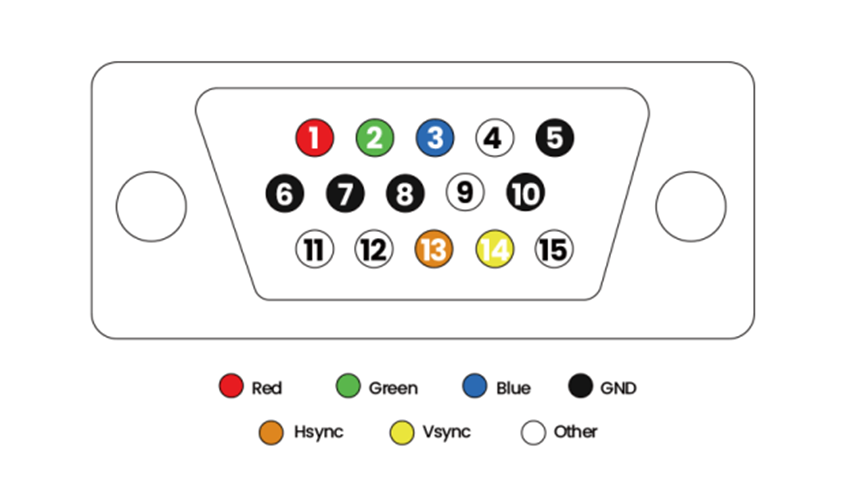
\includegraphics[width=0.5\linewidth]{VGA Connector Pins.png}
    \caption{VGA Connector Pins}
    \label{fig:VGA Pins}
\end{figure}

\section{Implementation}
\subsection{Block Diagram}

\begin{figure}[h!]
    \centering
    \includesvg[width=\textwidth]{vga_system.svg}
    \caption{System Block Diagram}
    \label{fig:block diagram}
\end{figure}

The top-level Vivado block diagram \cite{noauthor_vipinkmenonvga_nodate}\cite{noauthor_using_nodate} for the Zedboard’s VGA interface is designed to handle video data transfer, formatting, and timing generation. Central to this design is the ZYNQ7 Processing System (PS), which provides the high-level control and data management. A Clocking Wizard is used to generate stable, phase-aligned clock signals necessary for synchronous operation of all the video-related IP cores. To ensure proper system initialization, the Processor System Reset block manages resets for the entire design, thereby guaranteeing that all modules start in a known, consistent state.

At the heart of video data handling is the AXI Video Direct Memory Access (VDMA) core. The VDMA fetches frames from memory and converts them into a streaming video data format. This video stream is then processed by the Video Timing Controller, which provides all the necessary timing signals (horizontal and vertical sync, blanking) required by standard video interfaces. The combination of VDMA and VTC ensures that pixel data arrives at the correct time and in the proper sequence.

Once the properly timed video stream is available, the AXI4-Stream to Video Out IP core converts the AXI4-Stream video data into analog-friendly RGB signals that comply with the VGA protocol requirements [\cref{subsec:VGA Protocol}]Before these signals are presented at the VGA output pins, a multiplexer (mux[\cref{code:mux}]) and Slice IP cores are employed to select and route the desired portions of the data word to the \verb|VGA_R|, \verb|VGA_G|, and \verb|VGA_B|) lines. This final stage ensures that the correct pixel intensities reach the display.

\begin{listing}[H]
\begin{minted}[frame=lines]{verilog}
module mux(
input [23:0] i_data,
input i_control,
output [23:0] o_data
    );
assign o_data = (i_control==1)?i_data:24'h000000;
endmodule
\end{minted}
\caption{mux.v}
\label{code:mux}
\end{listing}

Together, these carefully orchestrated IP blocks create a streamlined, modular, and maintainable VGA output pipeline. Using standardized AXI interfaces and Xilinx-provided video IP cores, the design ensures compatibility, scalability, and simplicity with the VGA peripheral capabilities of the Zedboard.

\subsection{Program}

The Xilinx SDK was used to develop the software application \cite{noauthor_vipinkmenonvga_nodate} for using the VDMA IP and testing on the Zedboard.

\subsubsection{VDMA}

\begin{minted}[frame=lines]{c}
XAxiVdma_Config *config = XAxiVdma_LookupConfig(XPAR_AXI_VDMA_0_DEVICE_ID);
status = XAxiVdma_CfgInitialize(&myVDMA, config, config->BaseAddress);
\end{minted}
This section of the program is responsible for initializing the VDMA. \verb|XAxiVdma_LookupConfig| retrieves the DMA configuration based on the device ID and \verb|XAxiVdma_CfgInitialize| configures the VDMA hardware with this configuration.

\begin{minted}[frame=lines]{c}
ReadCfg.VertSizeInput = VSize;         // Vertical resolution: 1080
ReadCfg.HoriSizeInput = HSize * 3;     // Horizontal resolution in bytes: 1920 * 3 (RGB)
ReadCfg.Stride = HSize * 3;            // Bytes per row in the buffer
ReadCfg.EnableCircularBuf = 1;         // Circular buffer for continuous playback
ReadCfg.EnableSync = 1;                // Synchronization enabled
\end{minted}

This block sets the read channel parameters: \verb|VertSizeInput| and \verb|HoriSizeInput| specifies the vertical and horizontal size of the frame; \verb|Stride| indicates the number of bytes in one row; 

\verb|EnableCircularBuf| ensures that playback loops over the frames continuously; \verb|EnableSync| aligns the VDMA operations with the hardware.

\subsubsection{Frame Buffers Setup}

\begin{minted}[frame=lines]{c}
Addr = (u32)&Buffer[0];
for (Index = 0; Index < myVDMA.MaxNumFrames; Index++) {
    ReadCfg.FrameStoreStartAddr[Index] = Addr; // Set start address of each frame
    Addr += FrameSize;                         // Move to the next frame
}
status = XAxiVdma_DmaSetBufferAddr(&myVDMA, XAXIVDMA_READ, ReadCfg.FrameStoreStartAddr);
\end{minted}

This block sets up the frame buffers: each frame buffer's base address is set using the \verb|Buffer| array and \verb|FrameSize| (1080p frame size) is added to \verb|Addr| to calculate the next buffer's start address. These addresses are assigned to the VDMA using \verb|XAxiVdma_DmaSetBufferAddr|.

\subsubsection{Main Playback Loop}

\begin{minted}[frame=lines]{c}
while (1) {
    drawImage(HSize, VSize, imgHSize, imgVSize, (HSize - imgHSize) / 2, (VSize - imgVSize) / 2, images[imageIndex]);
    imageIndex = (imageIndex + 1) % NUM_IMAGES; // Cycle through images
    usleep(66666);
}
\end{minted}

This is the core playback loop where \verb|drawImage| Loads the current image into the buffer, centering it on the display. The \verb|imageIndex| is updated each loop to show the next image and loops back to the first image after the last.
\verb|usleep(66666)| adds a delay (\textasciitilde66 ms) to achieve approximately 15 frames per second.

\subsubsection{Drawing an Image}

\begin{minted}[frame=lines]{c}
int drawImage(u32 displayHSize, u32 displayVSize, u32 imageHSize, u32 imageVSize, 
              u32 hOffset, u32 vOffset, unsigned char *imagePointer) {
    for (int i = 0; i < displayVSize; i++) {
        for (int j = 0; j < displayHSize; j++) {
            if (i >= vOffset && i < vOffset + imageVSize && 
                j >= hOffset && j < hOffset + imageHSize) {
                int imageRow = i - vOffset;
                int imageCol = j - hOffset;
                int imageIndex = (imageRow * imageHSize + imageCol) * 3;

                Buffer[(i * displayHSize * 3) + (j * 3)] = imagePointer[imageIndex] / 16;       // R
                Buffer[(i * displayHSize * 3) + (j * 3) + 1] = imagePointer[imageIndex + 1] / 16; // G
                Buffer[(i * displayHSize * 3) + (j * 3) + 2] = imagePointer[imageIndex + 2] / 16; // B
            }
        }
    }
    Xil_DCacheFlushRange((UINTPTR)Buffer, FrameSize);
    return 0;
}
\end{minted}

The \verb|drawImage| function overlays an image onto a display buffer. It iterates over each pixel of the display, checking if it falls within the bounds of the image (based on \verb|hOffset| and \verb|vOffset|. If so, it maps the corresponding pixel from the image data, calculates its RGB values, and writes them into the \verb|Buffer| (global display memory), downscaling the color intensity by dividing each channel by 16 to match the 4 bit widths of the VGA color pins. The function ensures memory coherence by flushing the cache to physical memory using \verb|Xil_DCacheFlushRange|.

\subsubsection{Interrupt Setup}

\begin{minted}[frame=lines]{c}
Status = XScuGic_Connect(IntcInstancePtr, ReadIntrId, 
                          (Xil_InterruptHandler)XAxiVdma_ReadIntrHandler, 
                          (void *)AxiVdmaPtr);
if (Status != XST_SUCCESS) {
    xil_printf("Failed to connect interrupt controller\r\n");
    return XST_FAILURE;
}

XAxiVdma_SetCallBack(AxiVdmaPtr, XAXIVDMA_HANDLER_GENERAL, ReadCallBack, 
                     (void *)AxiVdmaPtr, XAXIVDMA_READ);
XAxiVdma_SetCallBack(AxiVdmaPtr, XAXIVDMA_HANDLER_ERROR, ReadErrorCallBack, 
                     (void *)AxiVdmaPtr, XAXIVDMA_READ);
\end{minted}

The code configures interrupt handling for the AXI VDMA (Video Direct Memory Access). It connects the interrupt controller to the VDMA's read interrupt using \verb|XScuGic_Connect|, linking it to the \verb|XAxiVdma_ReadIntrHandler| function and passing the VDMA instance context. If the connection fails, an error message is displayed, and the function exits. It also sets up two callback functions using \verb|XAxiVdma_SetCallBack|: one (\verb|ReadCallBack|) for general events like transfer completion and another (\verb|ReadErrorCallBack|) for handling errors. This setup ensures the system can respond appropriately to VDMA interrupts during operation.

\subsubsection{Buffer Generation}

Python was used to process and generate the \verb|video_buffers.h| file from an mp4 video [\cref{code:videoprocess} \cref{code:videobuffergen}]
Generating a \verb|video_buffers.h| header file

\begin{listing}[H]
    \begin{minted}[frame=lines]{c}
#ifndef IMAGE_BUFFERS_H
#define IMAGE_BUFFERS_H

#define imgHSize  640
#define imgVSize 360

#define NUM_IMAGES 3

// First frame (Red): Every pixel is (255, 0, 0)
unsigned char imageData1[imgHSize * imgVSize * 3] = {
    255, 0, 0, 255, 0, 0, 255, 0, 0, /*...*/, 255, 0, 0
};

// Second frame (Green): Every pixel is (0, 255, 0)
unsigned char imageData2[imgHSize * imgVSize * 3] = {
    0, 255, 0, 0, 255, 0, 0, 255, 0, /*...*/, 0, 255, 0
};

// Third frame (Blue): Every pixel is (0, 0, 255)
unsigned char imageData3[imgHSize * imgVSize * 3] = {
    0, 0, 255, 0, 0, 255, 0, 0, 255, /*...*/, 0, 0, 255
};

// Array of pointers to image buffers for convenience
unsigned char *images[] = {imageData1, imageData2, imageData3};

#endif // IMAGE_BUFFERS_H
    \end{minted}
\end{listing}
 
Each image is stored in flat arrays in row-major order, where every pixel is represented with 3 bytes (R, G, B). An array \verb|images| stores pointers to these buffers, allowing for easy access to each frame. 

\subsection{Result}

\begin{figure}[H]
    \centering
    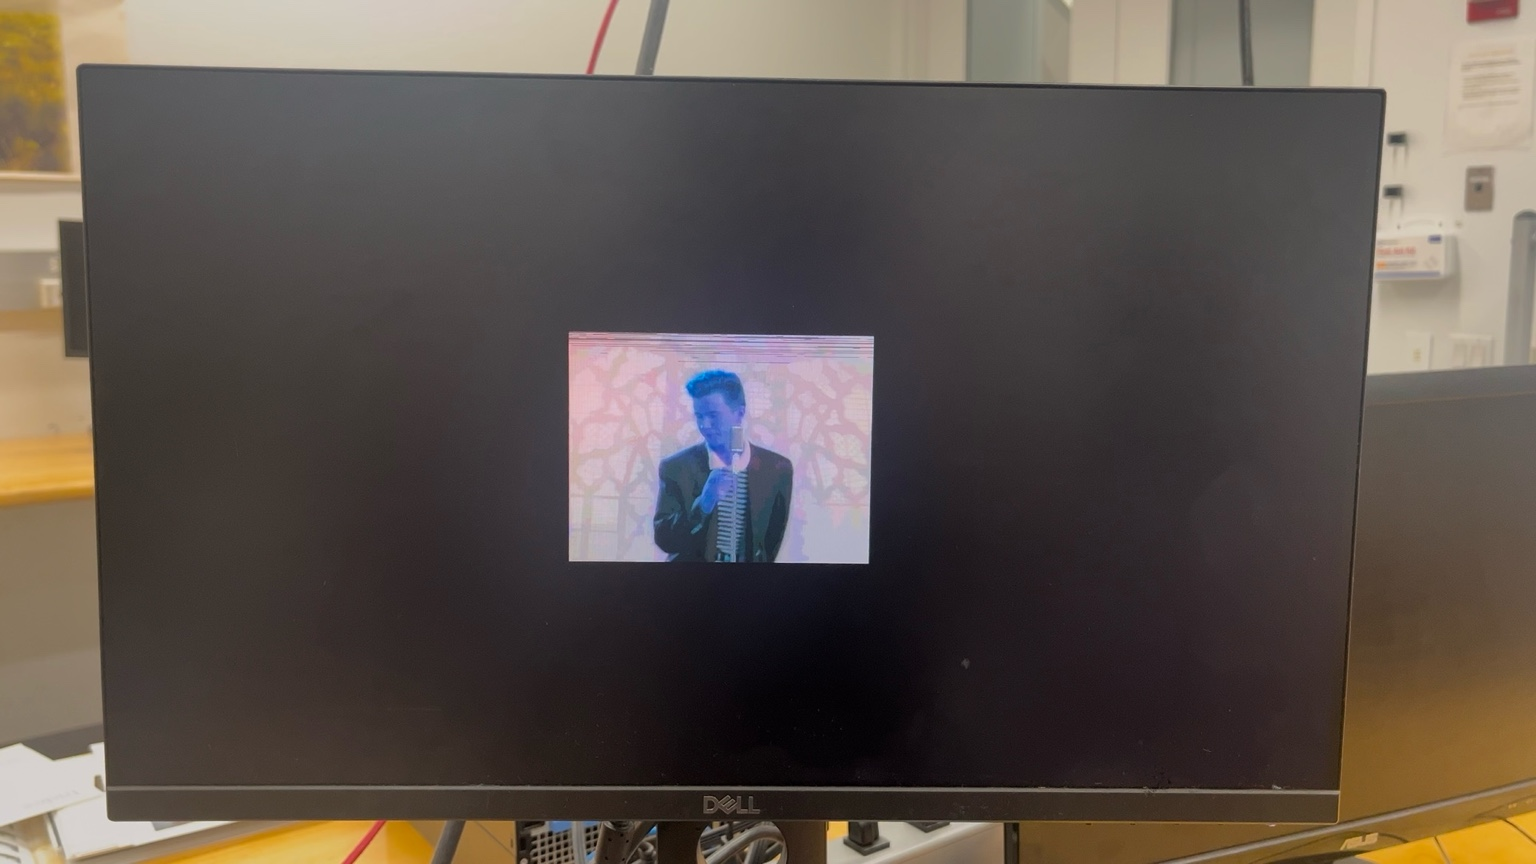
\includegraphics[width=1\linewidth]{rick_on_monitor.jpeg}
    \caption{Video on Monitor \cite{rick_astley_rick_2009}}
    \label{fig:rick}
\end{figure}

\section{Reflection}

\textit{What did you enjoy about this project?
What did you not like?
What was the hardest part?
What did you learn?}

I enjoyed strengthening my understanding of the AXI interface from the previous OLED project. This project required less hand-written verilog code as most of the IP cores that I needed were already developed and on the IP catalog. This made developing the block diagram both easier and harder as I didn't fully understand what was going on in the background of each IP core, but the high level abstraction made it much faster to get to the final product. As I mentioned in the reflection for the OLED project, I wanted to rely less on the Vipin tutorial for this project, and put more time into reading documentation directly from AMD, however, in the end I still developed the majority of this project with Vipin. As most of the VGA implementation was guided with Vipin, the most difficult part of this project was implementing the color video aspect. I used python to generate the video buffers in this project, but in the future I would like to use C code to extract the video buffers directly from an mp4 file.

\section{Appendix}

\begin{longlisting}
    \begin{minted}[frame=single, linenos]{c}
/*
 * display.c
 *
 *  Created on: Dec 13, 2024
 *      Author: jaeho.cho
 */

#include "xparameters.h"
#include "xaxivdma.h"
#include "xscugic.h"
#include "sleep.h"
#include <stdlib.h>
#include "xil_cache.h"
#include "video_buffers.h" // Include an array of image pointers

#define HSize 1920
#define VSize 1080
#define FrameSize HSize*VSize*3
//#define imgHSize 640
//#define imgVSize 360
//#define NUM_IMAGES 3

static XScuGic Intc;
static int SetupIntrSystem(XAxiVdma *AxiVdmaPtr, u16 ReadIntrId);
int drawImage(u32 displayHSize, u32 displayVSize, u32 imageHSize, u32 imageVSize, u32 hOffset, u32 vOffset, unsigned char *imagePointer);
void clearBuffer(unsigned char *buffer, u32 size);

unsigned char Buffer[FrameSize];

int main() {
    int status;
    int Index;
    u32 Addr;
    XAxiVdma myVDMA;
    XAxiVdma_Config *config = XAxiVdma_LookupConfig(XPAR_AXI_VDMA_0_DEVICE_ID);
    XAxiVdma_DmaSetup ReadCfg;

    status = XAxiVdma_CfgInitialize(&myVDMA, config, config->BaseAddress);
    if (status != XST_SUCCESS) {
        xil_printf("DMA Initialization failed\r\n");
        return XST_FAILURE;
    }

    ReadCfg.VertSizeInput = VSize;
    ReadCfg.HoriSizeInput = HSize * 3;
    ReadCfg.Stride = HSize * 3;
    ReadCfg.FrameDelay = 0;
    ReadCfg.EnableCircularBuf = 1;
    ReadCfg.EnableSync = 1;
    ReadCfg.PointNum = 0;
    ReadCfg.EnableFrameCounter = 0;
    ReadCfg.FixedFrameStoreAddr = 0;

    status = XAxiVdma_DmaConfig(&myVDMA, XAXIVDMA_READ, &ReadCfg);
    if (status != XST_SUCCESS) {
        xil_printf("Read channel config failed %d\r\n", status);
        return XST_FAILURE;
    }

    Addr = (u32)&Buffer[0];

    for (Index = 0; Index < myVDMA.MaxNumFrames; Index++) {
        ReadCfg.FrameStoreStartAddr[Index] = Addr;
        Addr += FrameSize;
    }

    status = XAxiVdma_DmaSetBufferAddr(&myVDMA, XAXIVDMA_READ, ReadCfg.FrameStoreStartAddr);
    if (status != XST_SUCCESS) {
        xil_printf("Read channel set buffer address failed %d\r\n", status);
        return XST_FAILURE;
    }

    XAxiVdma_IntrEnable(&myVDMA, XAXIVDMA_IXR_COMPLETION_MASK, XAXIVDMA_READ);

    SetupIntrSystem(&myVDMA, XPAR_FABRIC_AXI_VDMA_0_MM2S_INTROUT_INTR);

    status = XAxiVdma_DmaStart(&myVDMA, XAXIVDMA_READ);
    if (status != XST_SUCCESS) {
        xil_printf("DMA Start failed\r\n");
        return XST_FAILURE;
    }

    // Loop through images for video playback
    int imageIndex = 0;
    while (1) {
        // Load the current image into the buffer
        drawImage(HSize, VSize, imgHSize, imgVSize, (HSize - imgHSize) / 2, (VSize - imgVSize) / 2, images[imageIndex]);

        // Update the image index
        imageIndex = (imageIndex + 1) % NUM_IMAGES;

        // Wait for a short duration to simulate frame rate
        usleep(66666);
    }

    return 0;
}

/*****************************************************************************/
/* Call back function for read channel
******************************************************************************/

static void ReadCallBack(void *CallbackRef, u32 Mask) {
    xil_printf("Read Call back function is called\r\n");
}

/*****************************************************************************/
/* Error call back function
******************************************************************************/

static void ReadErrorCallBack(void *CallbackRef, u32 Mask) {
    xil_printf("Read Call back Error function is called\r\n");
}

/*****************************************************************************/
/* Setup Interrupt System
******************************************************************************/
static int SetupIntrSystem(XAxiVdma *AxiVdmaPtr, u16 ReadIntrId) {
    int Status;
    XScuGic *IntcInstancePtr = &Intc;

    XScuGic_Config *IntcConfig;
    IntcConfig = XScuGic_LookupConfig(XPAR_PS7_SCUGIC_0_DEVICE_ID);
    Status = XScuGic_CfgInitialize(IntcInstancePtr, IntcConfig, IntcConfig->CpuBaseAddress);
    if (Status != XST_SUCCESS) {
        xil_printf("Interrupt controller initialization failed\r\n");
        return XST_FAILURE;
    }

    Status = XScuGic_Connect(IntcInstancePtr, ReadIntrId, (Xil_InterruptHandler)XAxiVdma_ReadIntrHandler, (void *)AxiVdmaPtr);
    if (Status != XST_SUCCESS) {
        xil_printf("Failed to connect interrupt controller\r\n");
        return XST_FAILURE;
    }

    XScuGic_Enable(IntcInstancePtr, ReadIntrId);

    Xil_ExceptionInit();
    Xil_ExceptionRegisterHandler(XIL_EXCEPTION_ID_INT, (Xil_ExceptionHandler)XScuGic_InterruptHandler, (void *)IntcInstancePtr);
    Xil_ExceptionEnable();

    XAxiVdma_SetCallBack(AxiVdmaPtr, XAXIVDMA_HANDLER_GENERAL, ReadCallBack, (void *)AxiVdmaPtr, XAXIVDMA_READ);
    XAxiVdma_SetCallBack(AxiVdmaPtr, XAXIVDMA_HANDLER_ERROR, ReadErrorCallBack, (void *)AxiVdmaPtr, XAXIVDMA_READ);

    return XST_SUCCESS;
}

/*****************************************************************************/
/* Draw Image Function
******************************************************************************/
int drawImage(u32 displayHSize, u32 displayVSize, u32 imageHSize, u32 imageVSize, u32 hOffset, u32 vOffset, unsigned char *imagePointer) {
    for (int i = 0; i < displayVSize; i++) {
        for (int j = 0; j < displayHSize; j++) {
            if (i >= vOffset && i < vOffset + imageVSize && j >= hOffset && j < hOffset + imageHSize) {
                int imageRow = i - vOffset;
                int imageCol = j - hOffset;
                int imageIndex = (imageRow * imageHSize + imageCol) * 3;

                Buffer[(i * displayHSize * 3) + (j * 3)] = imagePointer[imageIndex] / 16;       // R
                Buffer[(i * displayHSize * 3) + (j * 3) + 1] = imagePointer[imageIndex + 1] / 16; // G
                Buffer[(i * displayHSize * 3) + (j * 3) + 2] = imagePointer[imageIndex + 2] / 16; // B
            }
        }
    }
    Xil_DCacheFlushRange((UINTPTR)Buffer, FrameSize);
    return 0;
}

/*****************************************************************************/
/* Clear Buffer Function
******************************************************************************/
void clearBuffer(unsigned char *buffer, u32 size) {
    for (u32 i = 0; i < size; i++) {
        buffer[i] = 0x00; // Set all bytes to black
    }
}
    \end{minted}
\caption{display.c}
\label{code:display}
\end{longlisting}

\begin{listing}[H]
    \begin{minted}[frame=single, linenos]{python}
import cv2

# Input and output file paths
input_video_path = "video.mp4"
output_video_path = "output_video.mp4"
frame_divisor = 5

# Open the input video
cap = cv2.VideoCapture(input_video_path)

# Get video properties
frame_width = int(cap.get(cv2.CAP_PROP_FRAME_WIDTH))
frame_height = int(cap.get(cv2.CAP_PROP_FRAME_HEIGHT))
fps = int(cap.get(cv2.CAP_PROP_FPS))  # Original FPS
total_frames = int(cap.get(cv2.CAP_PROP_FRAME_COUNT))  # Total number of frames in the input
fourcc = cv2.VideoWriter_fourcc(*'mp4v')  # Codec for MP4

# Define the VideoWriter for output
out = cv2.VideoWriter(output_video_path, fourcc, fps / frame_divisor, (frame_width, frame_height))

frame_count = 0
output_frame_count = 0  # Counter for output frames

while True:
    ret, frame = cap.read()
    if not ret:
        break  # End of video

    # Write every nth frame to the output video
    if frame_count % frame_divisor == 0:
        out.write(frame)
        output_frame_count += 1  # Increment output frame counter
    
    frame_count += 1

# Release resources
cap.release()
out.release()

# Print total frames
print(f"Total number of frames in the input video: {total_frames}")
print(f"Total number of frames in the output video: {output_frame_count}")
print(f"New video saved at {output_video_path}")
    \end{minted}
\caption{video\_process.py}
\label{code:videoprocess}
\end{listing}

\begin{longlisting}
    \begin{minted}[frame=single, linenos]{python}
import cv2
import numpy as np
from tqdm.notebook import tqdm

# Output header file name
header_file_name = "video_buffers.h"

# Video input file
video_file = "output_video.mp4"

# Frame dimensions
imgHSize = 640
imgVSize = 360

# Open the video file
cap = cv2.VideoCapture(video_file)

if not cap.isOpened():
    raise IOError("Error: Cannot open video file.")

frame_count = 0
buffers = []

frame_total = int(cap.get(cv2.CAP_PROP_FRAME_COUNT))

for _ in range(frame_total):
    ret, frame = cap.read()
    if not ret:
        break  # Exit the loop if no frames are left

    # Resize frame to desired dimensions
    frame = cv2.resize(frame, (imgHSize, imgVSize))

    # Convert the frame to raw pixel data (flattened array)
    raw_data = frame.flatten()

    # Add the frame's pixel data to the list
    buffers.append(raw_data)
    frame_count += 1

cap.release()

# Write the header file
with open(header_file_name, "w") as header_file:
    header_file.write("#ifndef IMAGE_BUFFERS_H\n")
    header_file.write("#define IMAGE_BUFFERS_H\n\n")
    header_file.write(f"#define imgHSize  {imgHSize}\n")
    header_file.write(f"#define imgVSize {imgVSize}\n\n")
    header_file.write(f"#define NUM_IMAGES {frame_count}\n\n")


    for i, buffer in enumerate(buffers):
        header_file.write(f"unsigned char imageData{i + 1}[imgHSize * imgVSize * 3] = {{\n")
        buffer_str = ", ".join(map(str, buffer))
        header_file.write(f"    {buffer_str}\n")
        header_file.write("};\n\n")

    header_file.write("// Array of pointers to image buffers for convenience\n")
    image_pointers = ", ".join([f"imageData{i + 1}" for i in range(frame_count)])
    header_file.write(f"unsigned char *images[] = {{{image_pointers}}};\n\n")

    header_file.write("#endif // IMAGE_BUFFERS_H\n")

print(f"Header file '{header_file_name}' generated successfully with {frame_count} frames.")
    \end{minted}
\caption{video\_buffer.py}
\label{code:videobuffergen}
\end{longlisting}

\printbibliography

\end{document}